% Intended LaTeX compiler: xelatex
\documentclass[aspectratio=169,10pt]{beamer}
\usepackage{graphicx}
\usepackage{longtable}
\usepackage{wrapfig}
\usepackage{rotating}
\usepackage[normalem]{ulem}
\usepackage{amsmath}
\usepackage{amssymb}
\usepackage{hyperref}
\usepackage{fontspec}
\usepackage{array}
\setsansfont{FiraSans-Regular.otf}[BoldFont=FiraSans-Bold.otf,ItalicFont=FiraSans-Italic.otf,BoldItalicFont=FiraSans-BoldItalic.otf]
\AtBeginDocument{\AtBeginSection[]{}}
\institute{Carpenter-Shen Lab, Purdue University}
\usetheme{moloch}
\author{Alán F. Muñoz}
\date{21 October 2026}
\title{Uncovering biological relationships through morphological profiling: The JUMP-Cell Painting dataset and tools}
\subtitle{FASEB: Organelle Cross-Talk in Cellular Homeostasis}
\hypersetup{
 pdfauthor={Alán F. Muñoz},
 pdftitle={Uncovering biological relationships through morphological profiling: The JUMP-Cell Painting dataset and tools},
 pdfkeywords={},
 pdfsubject={},
 pdfcreator={Emacs 30.2 (Org mode 9.7.11)}, 
 pdflang={English}}
\begin{document}

\maketitle
\section*{Conference draft}
\label{sec:org0000018}
\begin{frame}[label={sec:org0000001}]{What is Cell Painting?}
\begin{columns}[c,onlytextwidth]
\begin{column}{0.36\textwidth}
\begin{itemize}
\item A fluorescence microscopy assay for measuring cell morphology.
\item Six dyes reveal cellular structures across five imaging channels.
\item Shape, intensity and texture describe responses to genes and compounds.
\end{itemize}
\end{column}
\begin{column}{0.60\textwidth}
\centering
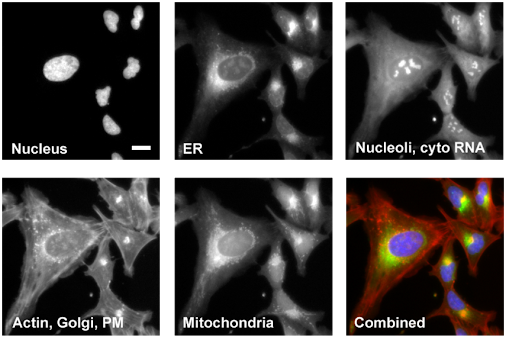
\includegraphics[width=0.98\linewidth,height=0.85\textheight,keepaspectratio]{assets/cell-painting-channels.png}
\end{column}
\end{columns}
\end{frame}
\begin{frame}[label={sec:org0000002}]{Cell Painting connects images to measurements}
\begin{center}
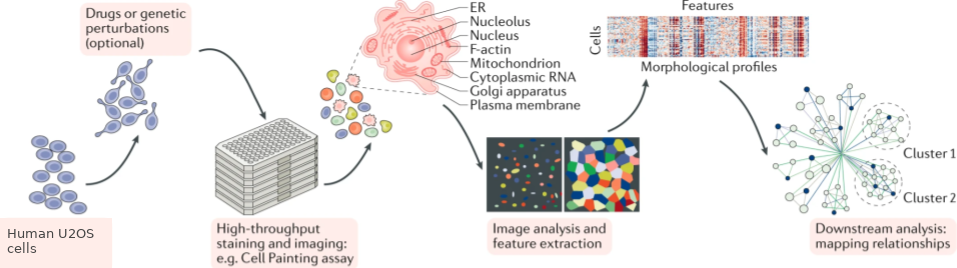
\includegraphics[keepaspectratio,width=0.99\linewidth,height=0.72\textheight]{assets/cell-painting.png}
\end{center}

\begin{itemize}
\item Stain and image cells, measure their appearance, and compare morphological profiles.
\end{itemize}
\end{frame}
\begin{frame}[label={sec:org0000003}]{Why turn images into profiles?}
Profiles summarize cellular appearance so we can compare and search large datasets.

\begin{columns}[T,onlytextwidth]
\begin{column}{0.48\textwidth}
\begin{block}{Engineered features: CellProfiler}
\begin{itemize}
\item Predefined measurements of size, shape, intensity, texture and spatial relationships.
\item Each feature has an explicit measurement definition.
\end{itemize}
\end{block}
\end{column}
\begin{column}{0.48\textwidth}
\begin{block}{Learned representations}
\begin{itemize}
\item Models learn visual features from training data using neural networks.
\item Images or cells are encoded as numerical feature vectors (embeddings).
\end{itemize}
\end{block}
\end{column}
\end{columns}
\medskip
\centering Compare perturbations $\cdot$ Group similar phenotypes $\cdot$ Prioritize follow-up
\end{frame}
\begin{frame}[label={sec:org0000004}]{Cells as vectors: useful does not always mean interpretable}
\begin{center}
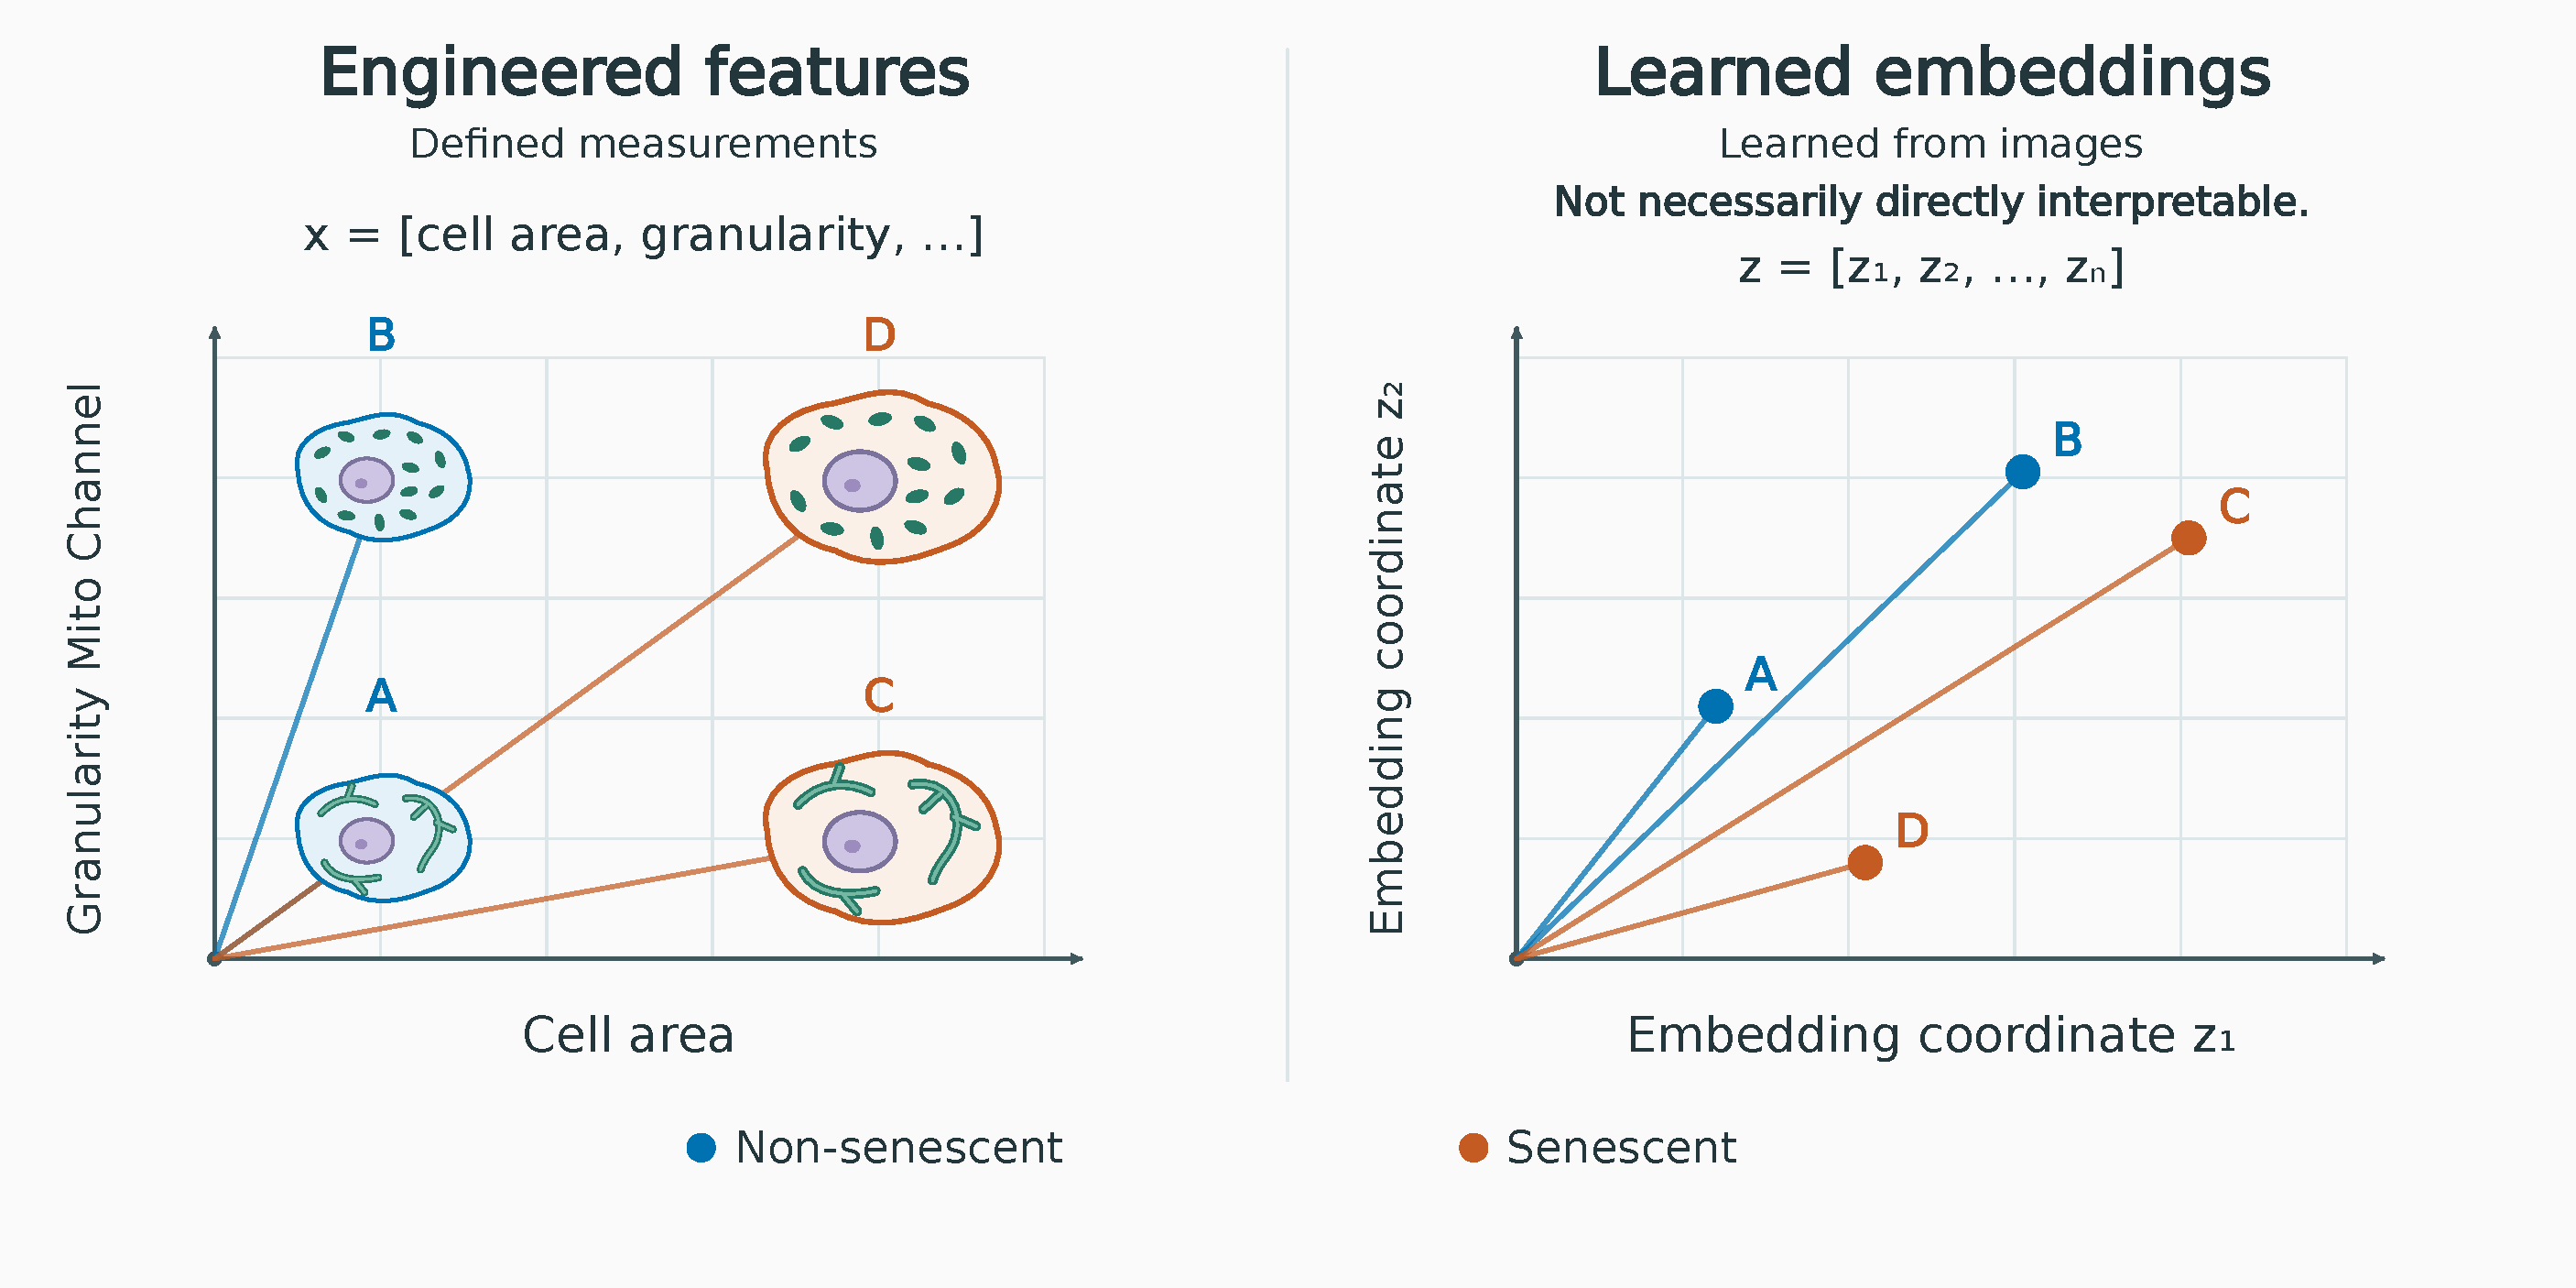
\includegraphics[keepaspectratio,width=0.99\linewidth,height=0.83\textheight]{assets/vector-interpretability.pdf}
\end{center}
\end{frame}
\begin{frame}[label={sec:org0000005}]{JUMP: Joint Undertaking for Morphological Profiling}
\begin{itemize}
\item A public Cell Painting dataset acquired across \alert{12 laboratories}, covering nearly 139,000 chemical and genetic perturbations.
\end{itemize}

\begin{center}
\fbox{\parbox[c][29mm][c]{0.27\linewidth}{\centering CRISPR knockout\par\medskip{\Large\bfseries 7,975}\par gene targets}}
\quad
\fbox{\parbox[c][29mm][c]{0.27\linewidth}{\centering\small Transient open reading frame (ORF) overexpression\par\smallskip{\Large\bfseries $\sim$12,600}\par genes}}
\quad
\fbox{\parbox[c][29mm][c]{0.27\linewidth}{\centering Compound treatment\par\medskip{\Large\bfseries 115,794}\par compounds}}
\end{center}

\begin{itemize}
\item Researchers can use the images, measurements and metadata to investigate their own questions.
\item Which gene, compound or phenotype from your lab would you like to explore?
\end{itemize}
\end{frame}
\begin{frame}[label={sec:org0000006}]{We make JUMP accessible via the JUMP Hub}
\begin{columns}[c,onlytextwidth]
\begin{column}{0.58\textwidth}
\centering
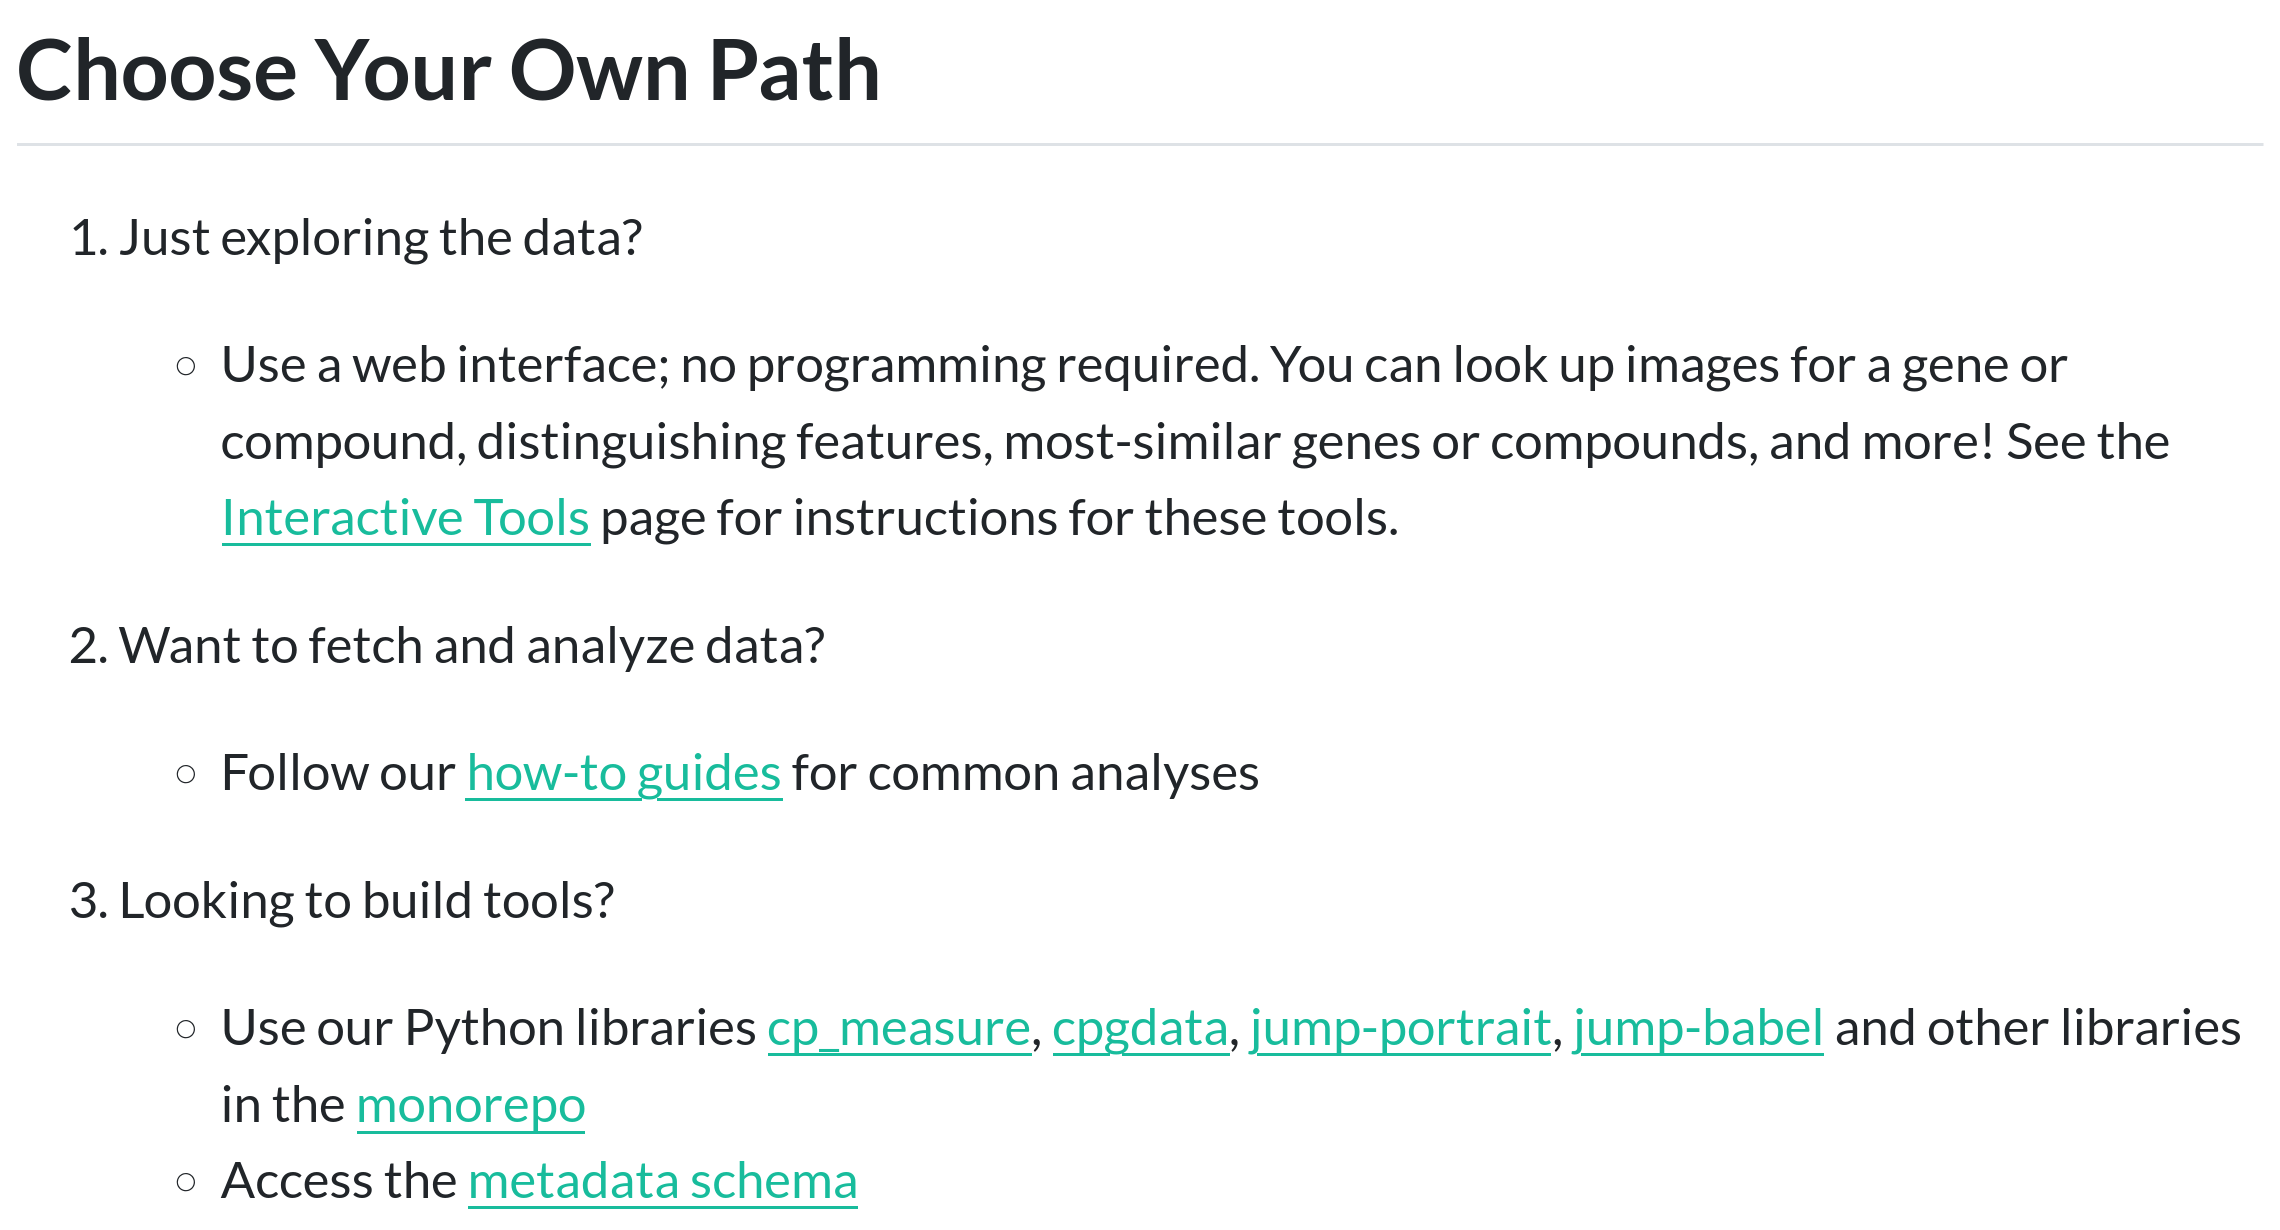
\includegraphics[width=0.98\linewidth,height=0.82\textheight,keepaspectratio]{assets/jump-hub-homepage.png}
\end{column}
\begin{column}{0.39\textwidth}
\begin{itemize}
\item Does my gene or compound have a Cell Painting phenotype?
\item Which perturbations produce related phenotypes?
\item What changes in the cells and their organelles?
\item Which cell subpopulations stand out?
\end{itemize}
\end{column}
\end{columns}
\end{frame}
\begin{frame}[label={sec:org0000007}]{Was my gene or compound tested?}
\begin{itemize}
\item Check whether your gene or compound is represented in JUMP.
\item Choose the perturbation: knockout, overexpression or compound treatment.
\item Open the associated profiles, images and experimental metadata.
\end{itemize}

\begin{center}
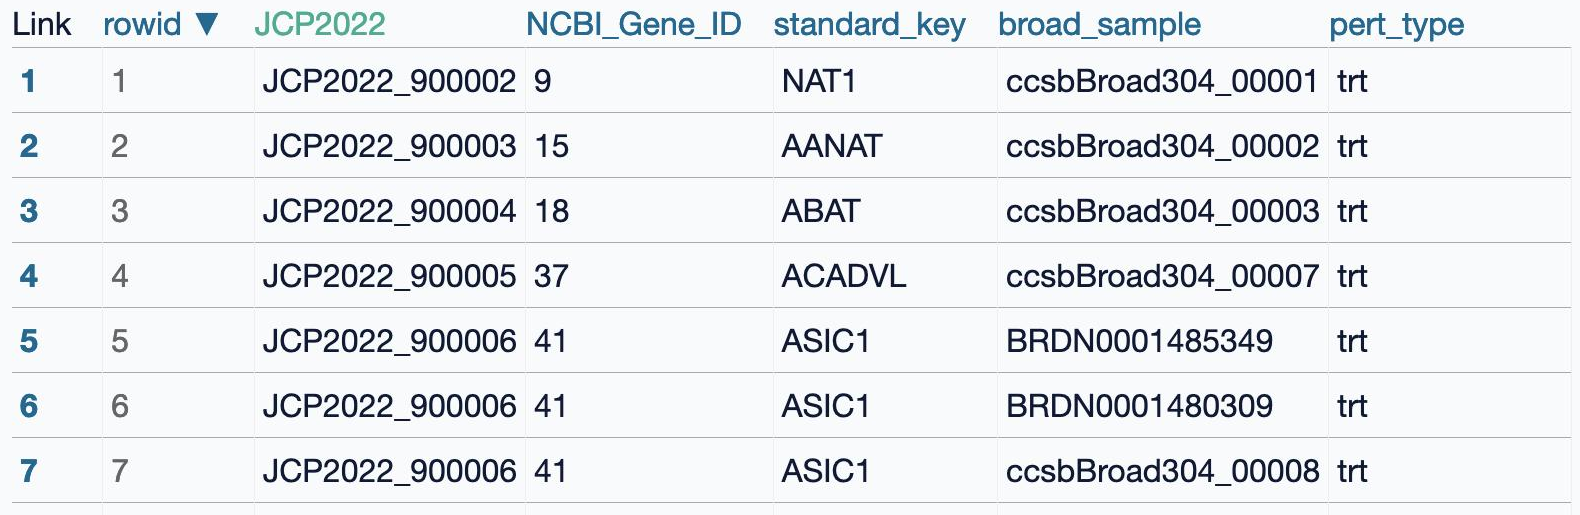
\includegraphics[keepaspectratio,width=0.90\linewidth,height=0.42\textheight]{assets/hub-identifiers.png}
\end{center}
\end{frame}
\begin{frame}[label={sec:org0000008}]{Which perturbations produce related phenotypes?}
\alert{MYT1 example}

\begin{center}
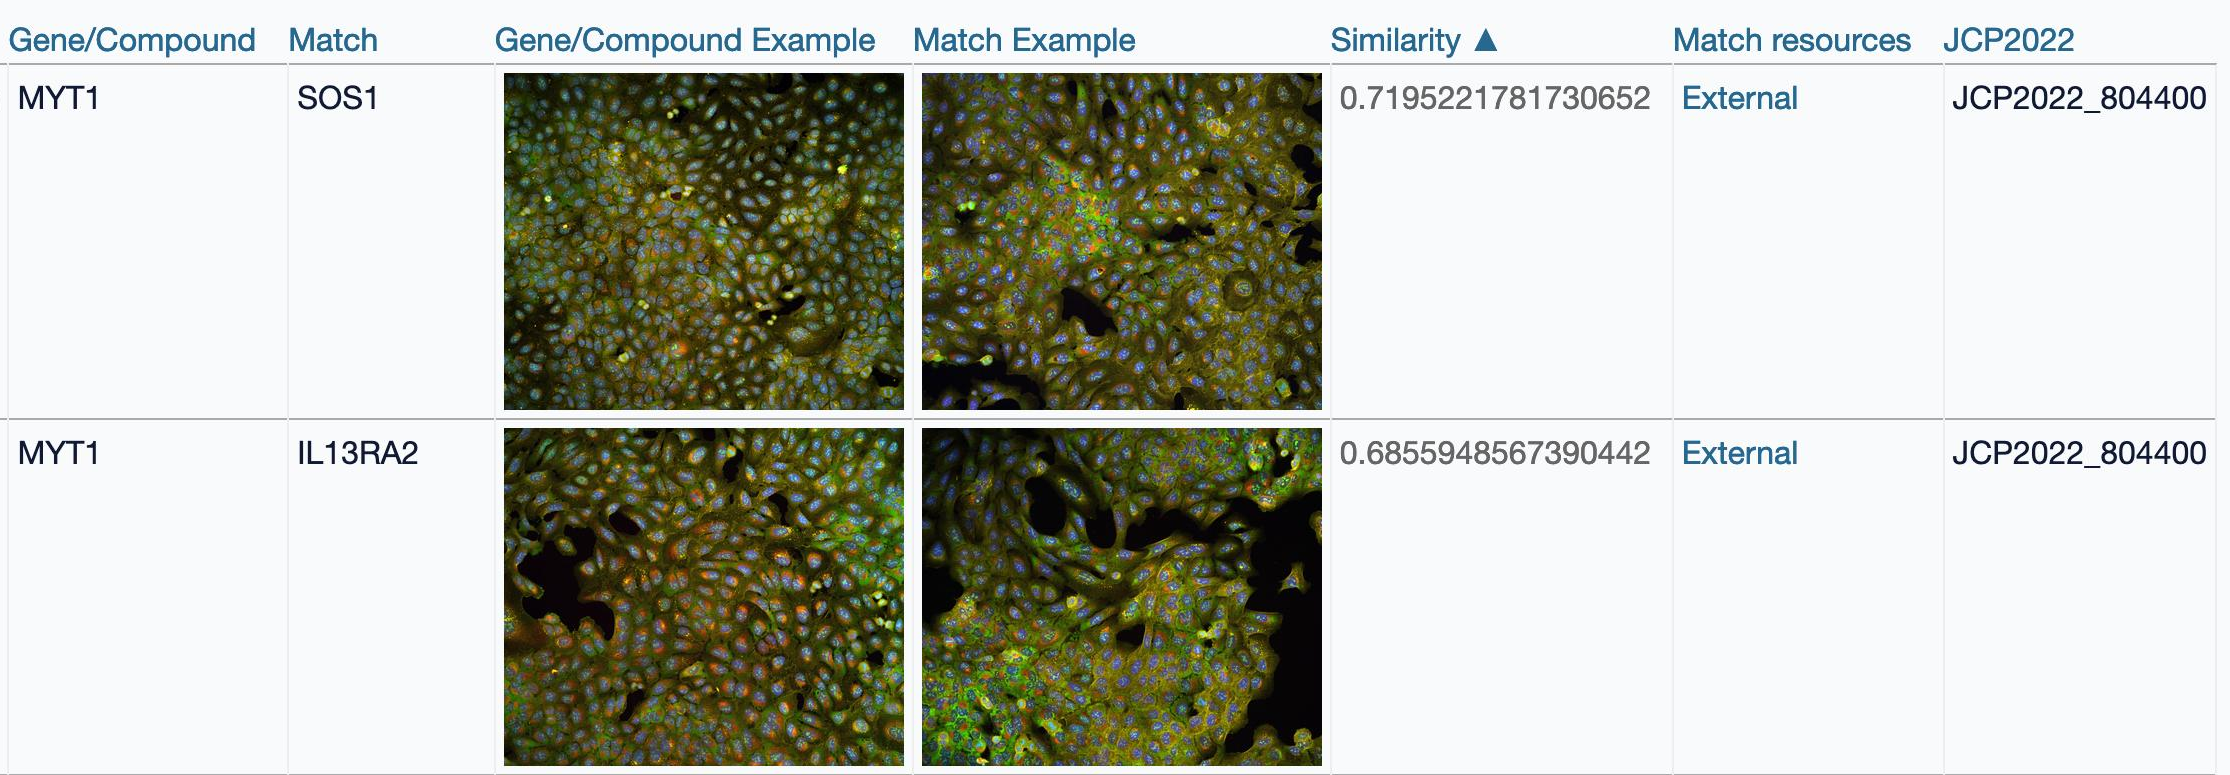
\includegraphics[keepaspectratio,width=0.93\linewidth,height=0.55\textheight]{assets/hub-matches.png}
\end{center}

\begin{itemize}
\item Explore the ranked matches to find candidates for follow-up.
\item Export the filtered list with its details using the table's JSON link.
\end{itemize}
\end{frame}
\begin{frame}[label={sec:org0000009}]{How does perturbing my gene change cell morphology?}
\alert{AVPR2 overexpression example}

\begin{center}
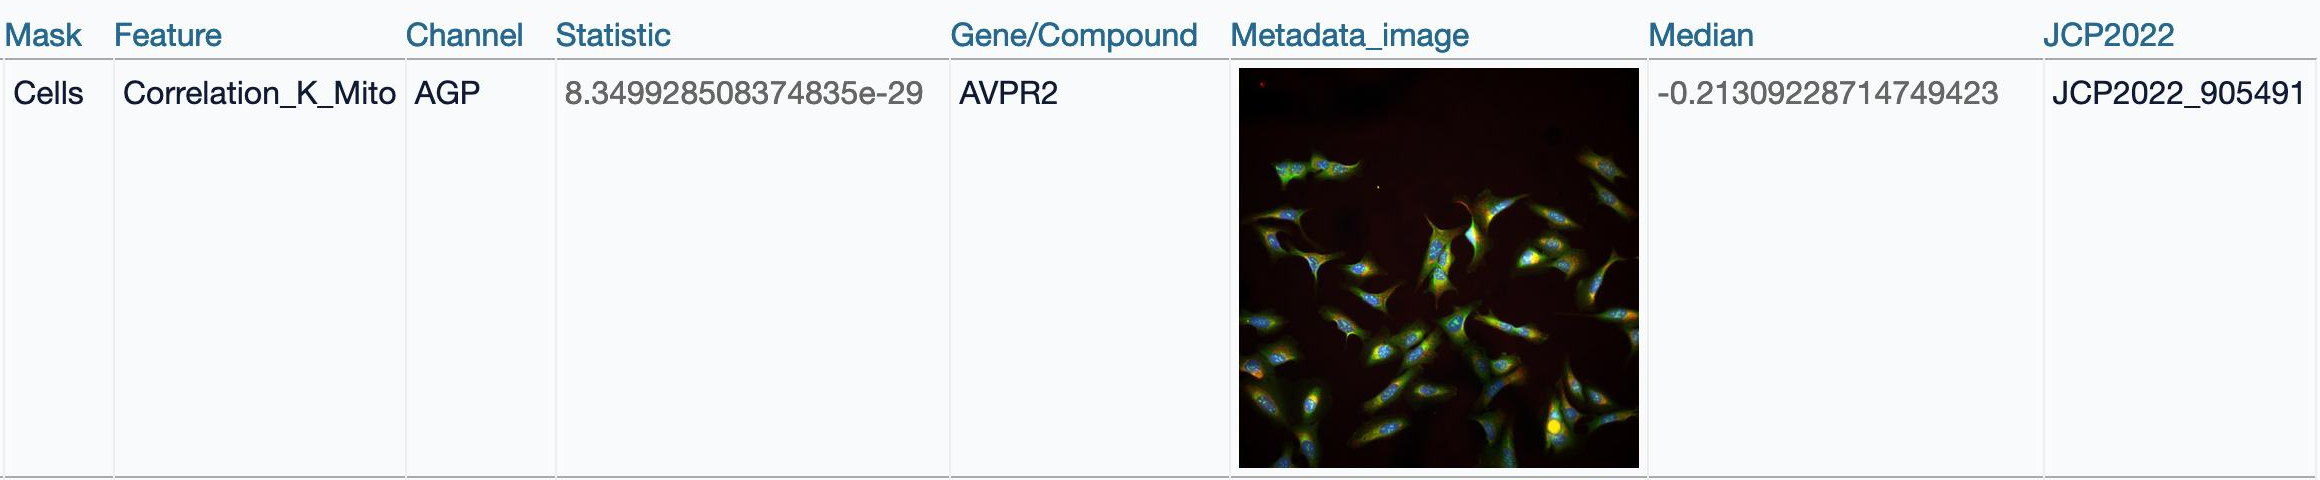
\includegraphics[keepaspectratio,width=0.98\linewidth,height=0.47\textheight]{assets/hub-features.png}
\end{center}

\begin{itemize}
\item A mitochondria--AGP overlap measurement stands out among the features.
\item Follow up by comparing mitochondrial distribution relative to actin, Golgi and plasma-membrane staining.
\end{itemize}
\end{frame}
\begin{frame}[label={sec:org000000a}]{Use JUMP as a screen for your phenotype}
\begin{columns}[T,onlytextwidth]
\begin{column}{0.46\textwidth}
\textbf{Measure many aspects of cell state}\par\medskip
\small
\begin{tabular}{@{}>{\raggedright\arraybackslash}p{0.32\linewidth}>{\raggedright\arraybackslash}p{0.60\linewidth}@{}}
\textbf{Size / shape} & Nuclear area, elongation \\[6pt]
\textbf{Intensity} & Mitochondrial staining \\[6pt]
\textbf{Texture} & Fine or coarse patterns \\[6pt]
\textbf{Correlation} & Relationships between channels \\[6pt]
\textbf{Distribution} & Peripheral or perinuclear signal
\end{tabular}
\end{column}
\begin{column}{0.50\textwidth}
\textbf{Which perturbations change nuclear size?}
\begin{itemize}
\item Select nuclear area in the feature table.
\item Rank perturbations by feature value and significance.
\item Inspect all available images for a perturbation.
\end{itemize}
\end{column}
\end{columns}
\end{frame}
\begin{frame}[label={sec:org000000b}]{What do the perturbed cells look like?}
\alert{MYT1 and PROZ gallery examples}

\begin{center}
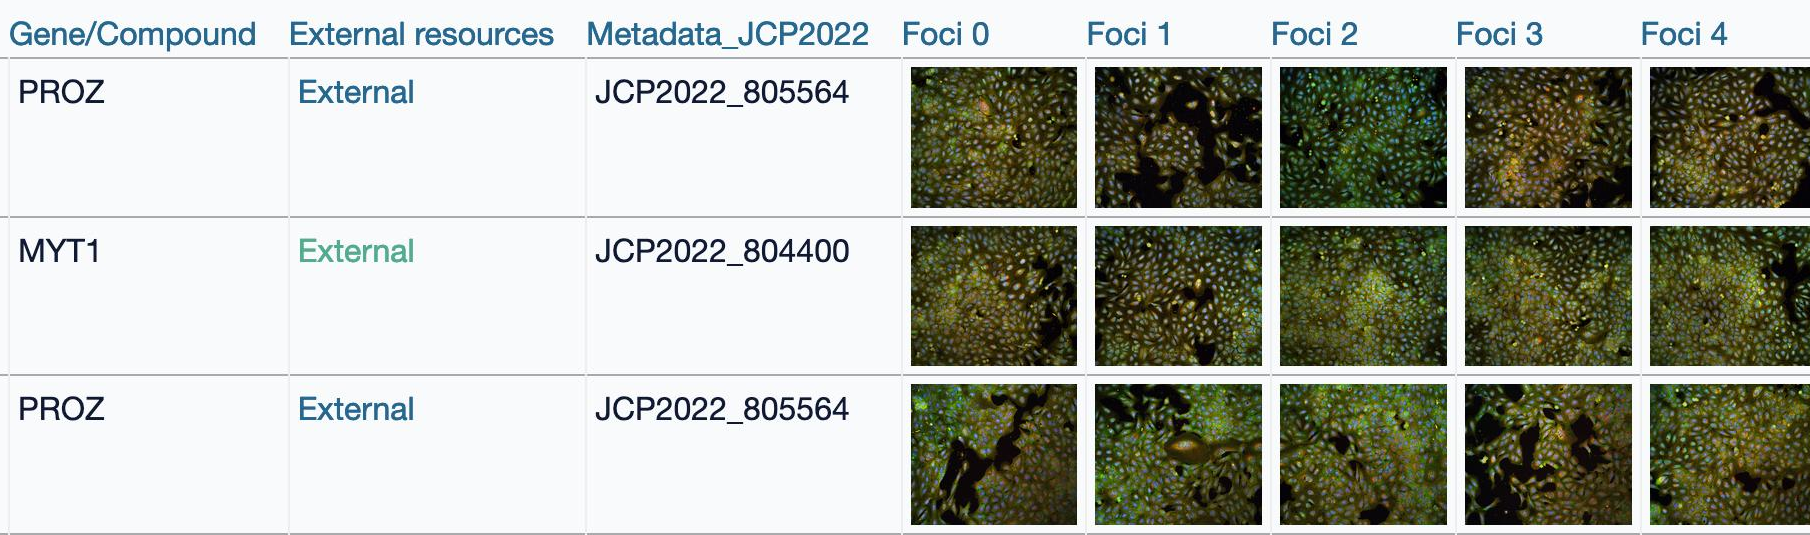
\includegraphics[keepaspectratio,width=0.93\linewidth,height=0.55\textheight]{assets/hub-gallery.png}
\end{center}

\begin{itemize}
\item Inspect cells across fields and imaging channels.
\item Retrieve the images and relevant controls for a closer comparison.
\end{itemize}
\end{frame}
\begin{frame}[label={sec:org000000c}]{Ask any AI assistant to explore the data for you, or build an interactive notebook}
\begin{quote}
Using the JUMP Hub documentation, write a notebook that links selected cells to their images and measurements. Include the source identifiers and save the analysis steps.
\end{quote}

\begin{itemize}
\item The tools and documentation we build for researchers can also be used by AI agents.
\item Biological expertise is essential for validating results.
\item Robust, reproducible tools help agents use consistent methods across analyses.
\item Extend the notebook with image models through nahual.
\end{itemize}
\end{frame}
\begin{frame}[label={sec:org000000d}]{Identify and explore cell subpopulations}
\alert{Interactive marimo notebook built from JUMP images and measurements}

\begin{center}
\href{https://doi.org/10.5281/zenodo.23462248}{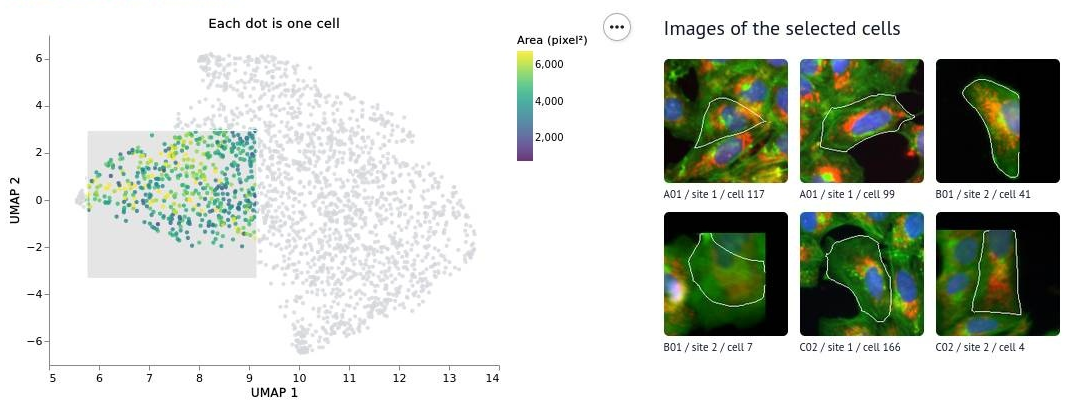
\includegraphics[width=0.96\linewidth,height=0.51\textheight,keepaspectratio]{assets/demo-selection-545.png}}
\end{center}

\begin{itemize}
\item Each dot is one of 2,223 cells from a JUMP Target-2 plate.
\item Select cells to update their images, area distribution and measurement summaries.
\end{itemize}
\end{frame}
\begin{frame}[label={sec:org000000e}]{How do cells in another region compare?}
\alert{The same notebook, with a second selection}

\begin{center}
\href{https://doi.org/10.5281/zenodo.23462248}{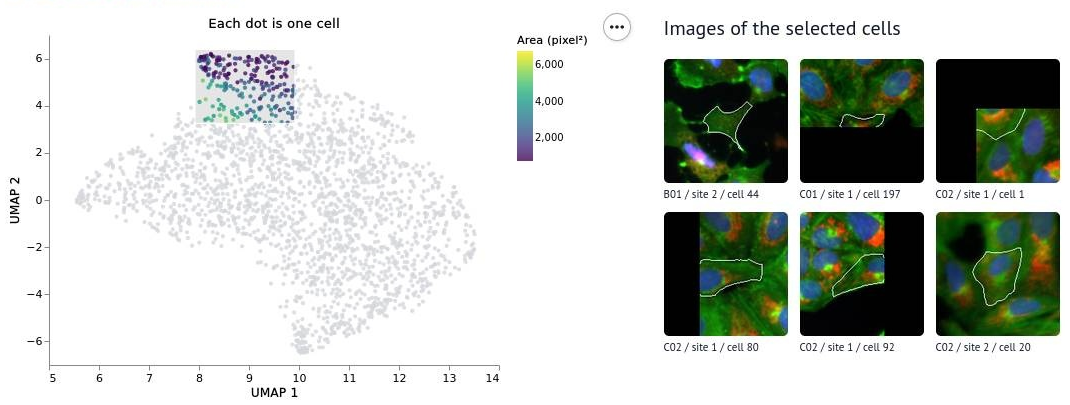
\includegraphics[width=0.96\linewidth,height=0.51\textheight,keepaspectratio]{assets/demo-selection-224.png}}
\end{center}

\begin{itemize}
\item Select another region: 224 cells in this example.
\item Compare cell images, areas and measurement summaries.
\item \href{https://doi.org/10.5281/zenodo.23462248}{Watch the recorded demo (23 s) on Zenodo}.
\end{itemize}
\end{frame}
\begin{frame}[label={sec:org000000f}]{Modern tools make image analysis more accessible}
\begin{tabular}{@{}>{\raggedright\arraybackslash}p{0.23\textwidth}>{\raggedright\arraybackslash}p{0.72\textwidth}@{}}
\textbf{Segmentation} & Cellpose: masks for cells and nuclei. \\[0.65em]
\textbf{Profiles} & cp\_measure: images and masks $\rightarrow$ quantitative profiles. \\[0.65em]
%\textbf{Learned features} & Generalist and specialised models that can be fine-tuned. \\[0.65em]
\textbf{Next-Generation data formats} & Parquet tables, Zarr arrays and JPEG XL image compression. \\[0.65em]
\textbf{Notebooks} & marimo: reactive notebooks and interactive apps. \\[0.65em]
\textbf{Python setup} & uv: fast package management, environments and lockfiles.
\end{tabular}\par\vspace{1em}
\centering\textbf{AI can turn these tools into workflows.}
\end{frame}
\begin{frame}[label={sec:org0000010}]{Nahual: swap models within one workflow}
\centering
{\Large\bfseries Swap models. Keep your workflow.}\par\bigskip
\renewcommand{\arraystretch}{1.8}
\begin{tabular}{@{}l l@{}}
\textbf{Image features} & \fbox{DINOv2}\ $\leftrightarrow$\ \fbox{DINOv3}\ $\leftrightarrow$\ \fbox{OpenPhenom}\ $\leftrightarrow$\ \fbox{MorphEm} \\
\textbf{Segmentation} & \fbox{Cellpose}\ $\leftrightarrow$\ \fbox{StarDist} \\
\textbf{Tracking} & \fbox{Trackastra}\ $\leftrightarrow$\ \fbox{Ultrack}
\end{tabular}
\end{frame}
\begin{frame}[label={sec:org0000011}]{Extract morphological profiles from your own images}
\begin{columns}[c,onlytextwidth]
\begin{column}{0.44\textwidth}
\centering
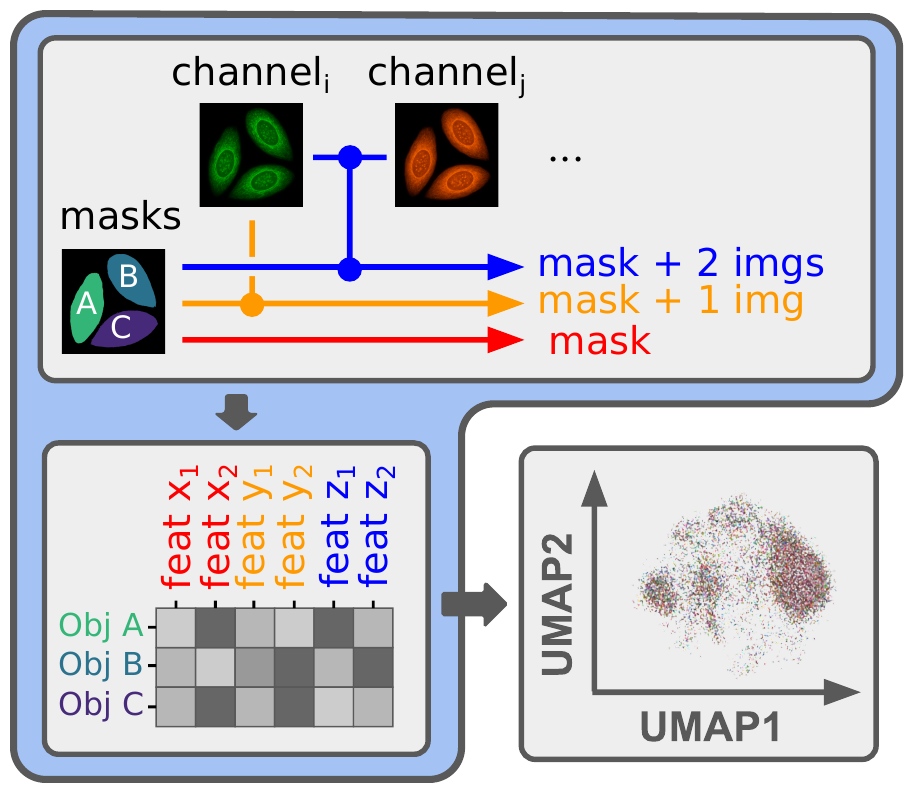
\includegraphics[width=0.98\linewidth,height=0.66\textheight,keepaspectratio]{assets/cp-measure-paper.png}
\end{column}
\begin{column}{0.53\textwidth}
\textbf{cp\_measure: feature extraction in Python}
\begin{itemize}
\item Build profiles of thousands of features across channels and cell compartments.
\item Integrate to your own Python pipelines.
\item Fastest software to obtain interpretable morphological features (>2x CellProfiler).
\end{itemize}
\end{column}
\end{columns}
\end{frame}
\begin{frame}[label={sec:org0000012}]{Developing new methods? Benchmark workflows with JUMP-lite}
\begin{center}
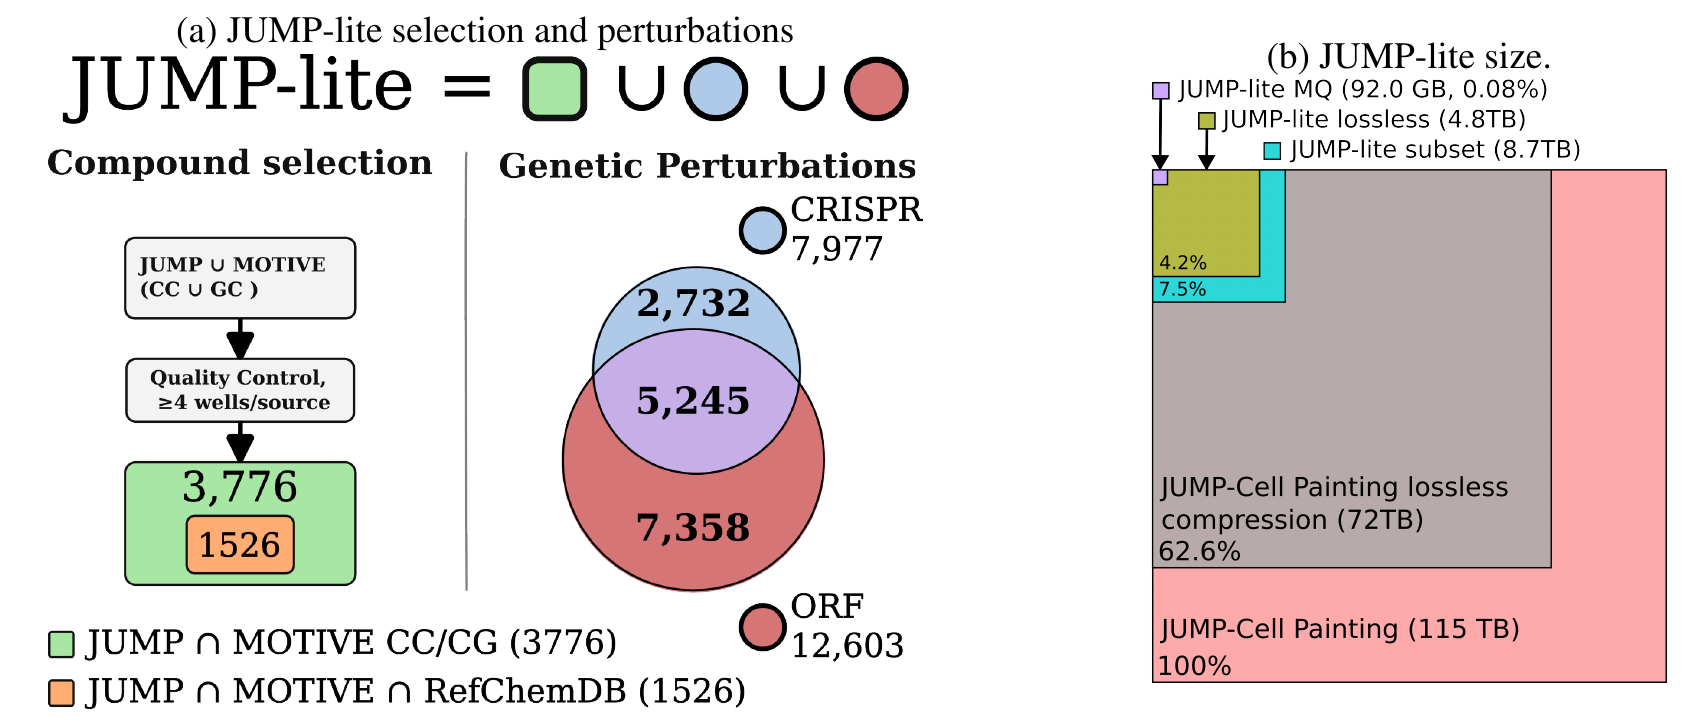
\includegraphics[keepaspectratio,width=0.96\linewidth,height=0.60\textheight]{assets/jump-lite-paper.png}
\end{center}

Use our compressed images to contrast your own vs the state-of-the-art.
\end{frame}
\begin{frame}[label={sec:org0000013}]{From lysosomal probes to spatial omics}
\begin{columns}[T,onlytextwidth]
\begin{column}{0.34\textwidth}
\begin{block}{Evaluate lysosomal probes}
\small Kenneth Li, University of Edinburgh\par
\normalsize
\begin{itemize}
\item Evaluate lysosomal acidification probes in cardiomyocytes.
\item Measure probe uptake, lysosomal localization and morphological changes over time.
\end{itemize}
\end{block}
\end{column}
\begin{column}{0.32\textwidth}
\begin{block}{Compare imaging modalities}
\small Minh Doan, GSK \par
\normalsize
\begin{itemize}
\item Compare bright-field, Cell Painting, cell-cycle and viability readouts.
\item Identify shared and complementary compound responses across assays.
\end{itemize}
\end{block}
\end{column}
\begin{column}{0.30\textwidth}
\begin{block}{Connect to spatial omics software}
\small Tim Treis, Helmholtz-Munich \par
\begin{itemize}
\item Integration of morphological features with Squidpy.
\end{itemize}
\end{block}
\end{column}
\end{columns}
\end{frame}
\begin{frame}[label={sec:org0000014}]{Take-home messages}
\begin{itemize}
\item Morphological profiles provide a quantitative representation of cell state.
\item We make JUMP data and query tools accessible to both researchers and AI agents.
\item We are building the foundations for agent-driven workflows that connect new microscopy images to quantitative insights.
\item Biological expertise is essential: experts remain in the loop to validate results.
\item Robust, reproducible tools help agents use consistent methods across analyses.
\end{itemize}
\end{frame}
\begin{frame}[label={sec:org0000015}]{Thank you}
\centering

\includegraphics[width=0.20\linewidth,height=0.08\textheight,keepaspectratio]{assets/broad-logo.png}\hspace{0.07\linewidth}

\includegraphics[width=0.24\linewidth,height=0.08\textheight,keepaspectratio]{assets/purdue-logo.png}\par\smallskip
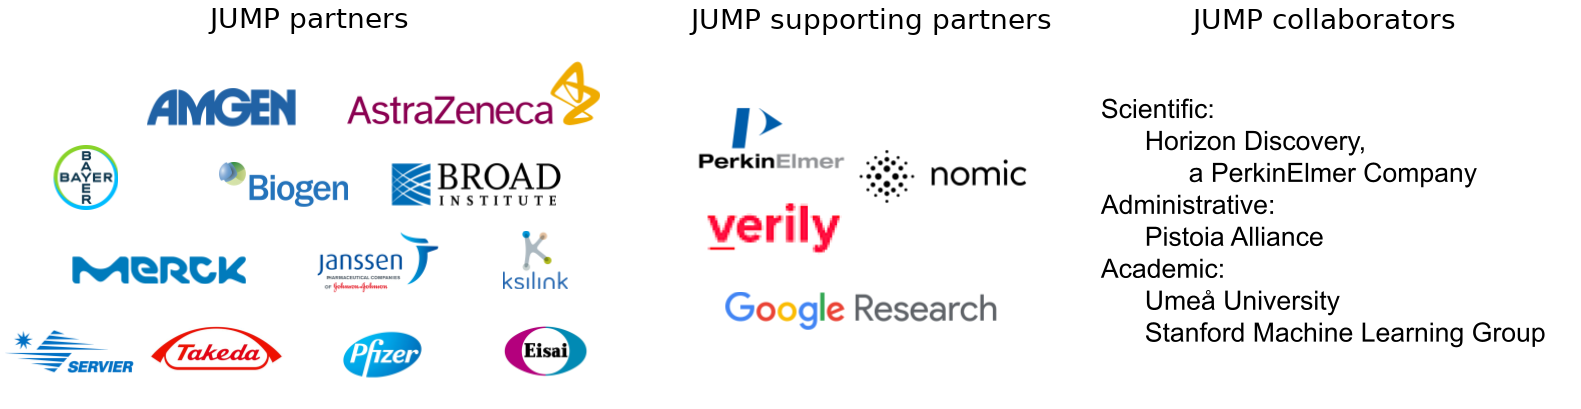
\includegraphics[width=0.98\linewidth,height=0.60\textheight,keepaspectratio]{assets/jump-partners.png}\par\medskip
{\small GSK provided part of the funding for this work.}\par
\end{frame}
\begin{frame}[label={sec:org0000016}]{References}
\begin{columns}[T,onlytextwidth]
\begin{column}{0.31\textwidth}
\small
\textbf{Assay and data}
\begin{itemize}
\item \href{https://doi.org/10.1038/nprot.2016.105}{Bray et al. (2016). Cell Painting.}\newline Nature Protocols.
\item \href{https://doi.org/10.1038/s41573-020-00117-w}{Chandrasekaran et al. (2021).}\newline Image-based profiling. Nature Reviews Drug Discovery.
\item \href{https://jump-cellpainting.broadinstitute.org/}{JUMP consortium}; \href{https://github.com/jump-cellpainting/datasets/tree/016e865fa0691244e0860943e41c7d6a88ed2580/metadata}{perturbation counts}; \href{https://github.com/broadinstitute/jump_hub/blob/e742f5aa37472eb17f326ba8315d22b27e58f330/explanations/data_description.md}{12 centers}.
\item \href{https://doi.org/10.1186/gb-2006-7-10-r100}{Carpenter et al. (2006). CellProfiler.}\newline Genome Biology.
\end{itemize}
\end{column}
\begin{column}{0.32\textwidth}
\small
\textbf{Analysis toolbox}
\begin{itemize}
\item \href{https://arxiv.org/abs/2608.07632v3}{Muñoz et al. (2026). JUMP-lite.}\newline \href{https://github.com/afermg/JUMP_lite}{Data and documentation}.
\item \href{https://arxiv.org/abs/2507.01163v1}{Muñoz et al. (2025). cp\_measure.}\newline \href{https://github.com/afermg/cp_measure}{Code}.
\item \href{https://github.com/MouseLand/cellpose}{Cellpose}: cell/nucleus segmentation.
\item \href{https://github.com/afermg/nahual}{Nahual}: image-model interfaces.
\item \href{https://squidpy.readthedocs.io/}{Squidpy}: spatial molecular and image analysis.
\end{itemize}
\end{column}
\begin{column}{0.31\textwidth}
\small
\textbf{Resources}
\begin{itemize}
\item \href{https://broadinstitute.github.io/jump_hub/}{JUMP Hub}: \href{https://broadinstitute.github.io/jump_hub/howto/interactive/1_jumprr_steps.html}{biological questions and table export}.
\item Recording: \href{https://github.com/afermg/JUMP_lite/blob/main/cpg_upload/TARGET2_ARTIFACTS_README.md}{JUMP Target-2 artifacts}.
\item \href{https://marimo.io/}{marimo}: reactive Python notebooks.
\item \href{https://docs.astral.sh/uv/}{uv}: Python environments and dependencies.
\end{itemize}
\end{column}
\end{columns}
\end{frame}
\begin{frame}[label={sec:org0000017}]{JUMP Hub and slides}
\begin{columns}[T,onlytextwidth]
\begin{column}{0.48\textwidth}
\centering
\href{https://broadinstitute.github.io/jump_hub/}{JUMP Hub}\par\smallskip
\href{https://broadinstitute.github.io/jump_hub/}{
\includegraphics[width=40mm]{assets/qr-jump-hub.png}}\par\smallskip
\href{https://broad.io/jump}{\texttt{broad.io/jump}}
\end{column}
\begin{column}{0.48\textwidth}
\centering
\href{https://github.com/afermg/2026_10_21_faseb_jump_hub/blob/main/slides.pdf}{Slides (PDF)}\par\smallskip
\href{https://github.com/afermg/2026_10_21_faseb_jump_hub/blob/main/slides.pdf}{
\includegraphics[width=40mm]{assets/qr-slides.png}}
\end{column}
\end{columns}
\end{frame}
\end{document}
